\documentclass{article}
\usepackage{array}
\usepackage[column=0]{cellspace}
\setlength\cellspacetoplimit{6pt}
\setlength\cellspacebottomlimit{6pt}
\usepackage{graphicx} % Required for inserting images
\usepackage{amsmath}
\usepackage{amssymb}
\usepackage{amsthm}
\usepackage{amsfonts}
\usepackage{gensymb}
\newcommand{\myvec}[1]{\ensuremath{\begin{pmatrix}#1\end{pmatrix}}}
\usepackage{graphicx}
\usepackage{mathtools}

\newcommand{\mydet}[1]{\ensuremath{\begin{vmatrix}#1\end{vmatrix}}}
\providecommand{\brak}[1]{\ensuremath{\left(#1\right)}}
\providecommand{\norm}[1]{\left\lVert#1\right\rVert}
\let\vec\mathbf

\title{MathConstruction}

\begin{document}

\section{NCERT 12.10.5.9}

Find the position vector of a point R which divides the line joining two points P and Q whose Position Vectors are $2\overrightarrow{a}+\overrightarrow{b}$ and $\overrightarrow{a}-3\overrightarrow{b}$ externally in the ration $1:2$.Also, Show that P is the mid point of the line segment BC \\
\textbf{Solution:}
The coordinates and ratio are given as
\begin{table}[h]
    \centering
    \begin{tabular}{|c|c|}
        \hline
        \textbf{Symbol} & \textbf{Value} \\
        \hline
        $\vec{P}$ & $2\overrightarrow{a}+\overrightarrow{b}$ \\
        \hline
        $\vec{Q}$ & $\overrightarrow{a}-3\overrightarrow{b}$ \\
        \hline
        n & $\frac{2}{1}$ \\
        \hline
    \end{tabular}
    \label{tab:mytable}
\end{table}
Using section formula
\begin{align}
    \vec{R}=\frac{Q-n.P}{1-n}\\
    \vec{R}=\frac{(\overrightarrow{a}-3\overrightarrow{b})-2(2\overrightarrow{a}+\overrightarrow{b})}{1-2}\\
    \vec{R}=3\overrightarrow{a}+5\overrightarrow{b}
\end{align}
\begin{table}[h]
    \centering
    \begin{tabular}{|c|c|}
        \hline
        \textbf{Symbol} & \textbf{Value}  \\
        \hline
        $\Vec{R}$ & $3\overrightarrow{a}+5\overrightarrow{b}$  \\
        \hline
    \end{tabular}
    \label{tab:mytable}
\end{table}
\begin{figure}[!ht]
    \centering
    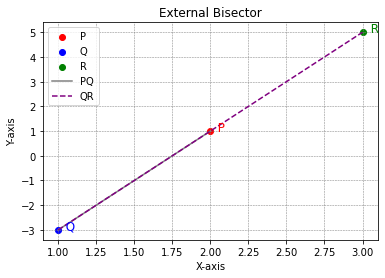
\includegraphics[width=\columnwidth]{/sdcard/geometry/math_computing/mathconstruction-2.png}
    \caption{point vectors P,Q,R}
    \label{fig:enter-label}
\end{figure}
\end{document}
